\documentclass[12pt,titlepage]{extarticle}
% Document Layout and Font
\usepackage{subfiles}
\usepackage[margin=2cm, headheight=15pt]{geometry}
\usepackage{fancyhdr}
\usepackage{enumitem}	
\usepackage{wrapfig}
\usepackage{float}
\usepackage{multicol}

\usepackage[p,osf]{scholax}

\renewcommand*\contentsname{Table of Contents}
\renewcommand{\headrulewidth}{0pt}
\pagestyle{fancy}
\fancyhf{}
\fancyfoot[R]{$\thepage$}
\setlength{\parindent}{0cm}
\setlength{\headheight}{17pt}
\hfuzz=9pt

% Figures
\usepackage{svg}

% Utility Management
\usepackage{color}
\usepackage{colortbl}
\usepackage{xcolor}
\usepackage{xpatch}
\usepackage{xparse}

\definecolor{gBlue}{HTML}{7daea3}
\definecolor{gOrange}{HTML}{e78a4e}
\definecolor{gGreen}{HTML}{a9b665}
\definecolor{gPurple}{HTML}{d3869b}

\definecolor{links}{HTML}{1c73a5}
\definecolor{bar}{HTML}{584AA8}

% Math Packages
\usepackage{mathtools, amsmath, amsthm, thmtools, amssymb, physics}
\usepackage[scaled=1.075,ncf,vvarbb]{newtxmath}

\newcommand\B{\mathbb{C}}
\newcommand\C{\mathbb{C}}
\newcommand\R{\mathbb{R}}
\newcommand\Q{\mathbb{Q}}
\newcommand\N{\mathbb{N}}
\newcommand\Z{\mathbb{Z}}

\DeclareMathOperator{\lcm}{lcm}

% Probability Theory
\newcommand\Prob[1]{\mathbb{P}\qty(#1)}
\newcommand\Var[1]{\text{Var}\qty(#1)}
\newcommand\Exp[1]{\mathbb{E}\qty[#1]}

% Analysis
\newcommand\ball[1]{\B\qty(#1)}
\newcommand\conj[1]{\overline{#1}}
\DeclareMathOperator{\Arg}{Arg}
\DeclareMathOperator{\cis}{cis}

% Linear Algebra
\DeclareMathOperator{\dom}{dom}
\DeclareMathOperator{\range}{range}
\DeclareMathOperator{\spann}{span}
\DeclareMathOperator{\nullity}{nullity}

% TIKZ
\usepackage{tikz}
\usepackage{pgfplots}
\usetikzlibrary{arrows.meta}
\usetikzlibrary{math}
\usetikzlibrary{cd}

% Boxes and Theorems
\usepackage[most]{tcolorbox}
\tcbuselibrary{skins}
\tcbuselibrary{breakable}
\tcbuselibrary{theorems}

\newtheoremstyle{default}{0pt}{0pt}{}{}{\bfseries}{\normalfont.}{0.5em}{}
\theoremstyle{default}

\renewcommand*{\proofname}{\textit{\textbf{Proof.}}}
\renewcommand*{\qedsymbol}{$\blacksquare$}
\tcolorboxenvironment{proof}{
	breakable,
	coltitle = black,
	colback = white,
	frame hidden,
	boxrule = 0pt,
	boxsep = 0pt,
	borderline west={3pt}{0pt}{bar},
	% borderline west={3pt}{0pt}{gPurple},
	sharp corners = all,
	enhanced,
}

\newtheorem{theorem}{Theorem}[section]{\bfseries}{}
\tcolorboxenvironment{theorem}{
	breakable,
	enhanced,
	boxrule = 0pt,
	frame hidden,
	coltitle = black,
	colback = blue!7,
	% colback = gBlue!30,
	left = 0.5em,
	sharp corners = all,
}

\newtheorem{corollary}{Corollary}[section]{\bfseries}{}
\tcolorboxenvironment{corollary}{
	breakable,
	enhanced,
	boxrule = 0pt,
	frame hidden,
	coltitle = black,
	colback = white!0,
	left = 0.5em,
	sharp corners = all,
}

\newtheorem{lemma}{Lemma}[section]{\bfseries}{}
\tcolorboxenvironment{lemma}{
	breakable,
	enhanced,
	boxrule = 0pt,
	frame hidden,
	coltitle = black,
	colback = green!7,
	left = 0.5em,
	sharp corners = all,
}

\newtheorem{definition}{Definition}[section]{\bfseries}{}
\tcolorboxenvironment{definition}{
	breakable,
	coltitle = black,
	colback = white,
	frame hidden,
	boxsep = 0pt,
	boxrule = 0pt,
	borderline west = {3pt}{0pt}{orange},
	% borderline west = {3pt}{0pt}{gOrange},
	sharp corners = all,
	enhanced,
}

\newtheorem{example}{Example}[section]{\bfseries}{}
\tcolorboxenvironment{example}{
	% title = \textbf{Example},
	% detach title,
	% before upper = {\tcbtitle\quad},
	breakable,
	coltitle = black,
	colback = white,
	frame hidden,
	boxrule = 0pt,
	boxsep = 0pt,
	borderline west={3pt}{0pt}{green!70!black},
	% borderline west={3pt}{0pt}{gGreen},
	sharp corners = all,
	enhanced,
}

\newtheoremstyle{remark}{0pt}{4pt}{}{}{\bfseries\itshape}{\normalfont.}{0.5em}{}
\theoremstyle{remark}
\newtheorem*{remark}{Remark}


% TColorBoxes
\newtcolorbox{week}{
	colback = black,
	coltext = white,
	fontupper = {\large\bfseries},
	width = 1.2\paperwidth,
	size = fbox,
	halign upper = center,
	center
}

\newcommand{\banner}[2]{
    \pagebreak
    \begin{week}
   		\section*{#1}
    \end{week}
    \addcontentsline{toc}{section}{#1}
    \addtocounter{section}{1}
    \setcounter{subsection}{0}
}

% Hyperref
\usepackage{hyperref}
\hypersetup{
	colorlinks=true,
	linktoc=all,
	linkcolor=links,
	bookmarksopen=true
}

% Error Handling
\PackageWarningNoLine{ExtSizes}{It is better to use one of the extsizes 
                          classes,^^J if you can}


\def\homeworknumber{5}
\fancyhead[R]{\textbf{Math 140A: Homework \#\homeworknumber}}
\fancyhead[L]{Eli Griffiths}
\renewcommand{\headrulewidth}{1pt}
\setlength\parindent{0pt}


% 10.2: 1,3,9,21,
% 10.3: 3,11
% 10.4: 1,3,5
% 10.5: 1,3,5
% 10.6: 3
% 11.1: 1,3,7,17
% 11.4: 1,3,5
% 11.5: 1
% 12.1: 5,15,23
% 12.2: 1,3,5
% 12.3: 5

\begin{document}

\subsection*{10.2.1}
There are 6 vertices and 6 edges.
\begin{center}
    \begin{tabular}{c|ccc}
        v & $\deg(v)$ & Isolated? & Pendant? \\\hline
        $a$ & $2$ &  & \\
        $b$ & $4$ & & \\
        $c$ & $1$ & & Y \\
        $d$ & $0$ & Y & \\
        $e$ & $2$ & & \\
        $f$ & $3$ & & \\
    \end{tabular}
\end{center}

\subsection*{10.2.3}
There are 9 vertices and 12 edges.
\begin{center}
    \begin{tabular}{c|ccc}
        v & $\deg(v)$ & Isolated? & Pendant? \\\hline
        $a$ & $3$ &  & \\
        $b$ & $2$ & & \\
        $c$ & $4$ & & \\
        $d$ & $0$ & Y & \\
        $e$ & $6$ & & \\
        $f$ & $0$ & Y & \\
        $g$ & $4$ & & \\
        $h$ & $2$ & & \\
        $i$ & $3$ & & \\
    \end{tabular}
\end{center}

\subsection*{10.2.9}
The are 5 vertices and 13 edges.
\begin{center}
    \begin{tabular}{c|ccc}
        v & $\deg^-(v)$ & $\deg^+(v)$ \\\hline
        $a$ & $6$ & $1$ \\
        $b$ & $1$ & $5$ \\
        $c$ & $2$ & $5$ \\
        $d$ & $4$ & $2$ \\
        $e$ & $0$ & $0$
    \end{tabular}
\end{center}

\subsection*{10.2.21}
It is bipartite since you can assign say blue to $e$ and red to the rest of the vertices and there will be no adjacent colorings.

\subsection*{10.3.3}
\[
    \begin{array}{c|c}
        v & N(v) \\\hline
        a & \qty{a,b,c,d} \\
        b & \qty{d} \\
        c & \qty{a,b} \\
        d & \qty{b, c, d}
    \end{array}
\]

\subsection*{10.3.11}
\begin{center}
    \begin{tikzpicture}[scale=2]
      \tikzstyle{vertex}=[circle,draw=black,line width=1pt,minimum size=20pt,inner sep=2pt]
      \tikzstyle{edge}=[->, thick]
      \tikzstyle{bnd}=[bend right=10]
      \node[vertex] (a) at (-1,1) {$a$};
      \node[vertex] (b) at (1,1) {$b$};
      \node[vertex] (c) at (-1,-1) {$c$};
      \node[vertex] (d) at (1,-1) {$d$};
      \draw[edge] (a) to [bnd] (c);
      \draw[edge] (c) to [bnd] (a);
      \draw[edge] (a) to [bnd] (d);
      \draw[edge] (d) to [bnd] (a);
      \draw[edge] (b) to [bnd] (c);
      \draw[edge] (c) to [bnd] (b);
      \draw[edge] (c) to [bnd] (d);
      \draw[edge] (d) to [bnd] (c);
      \draw[edge] (d) to [bnd] (b);
    \end{tikzpicture}
\end{center}

\subsection*{10.4.1}
\begin{tasks}
    \task Path of length 4 that isnt a circuit or simple
    \task Not a path
    \task Not a path
    \task Path of length 5 that is a circuit
\end{tasks}

\subsection*{10.4.3}
Not connected

\subsection*{10.4.5}
Not connected

\subsection*{10.5.1}
No euler path or circuit exists

\subsection*{10.5.3}
No euler circuit exists, but there is an euler path $a \to e \to c \to e \to b \to e \to d \to b \to a \to c \to d$

\subsection*{10.5.5}
$a \to b \to c \to d \to c \to e \to d \to b \to e \to a \to e \to a$

\subsection*{10.6.3}
The path $a \to c \to d \to e \to g \to z$ is a shortest path of length 16.

\subsection*{11.1.1}
$a,c$ and $e$ are trees.

\subsection*{11.1.3}
\begin{tasks}
    \task $a$
    \task $a,b,c,d,f,h,j,q,t$
    \task $e,l,m,n,g,o,p,i,s,u,r,k$
    \task $q,r$
    \task $c$
    \task $p$
    \task $f,b,a$
    \task $e,f,l,m,n$
\end{tasks}

\subsection*{11.1.7}
\[
    \begin{array}{c|l}
        \text{Level} & L(V) \\\hline
        0 & a \\
        1 & b,c,d \\
        2 & e,f,g,h,i,j,k \\
        3 & l,m,n,o,p,q,r \\
        4 & s,t \\
        5 & u
    \end{array}
\]

\subsection*{11.1.17}
A tree with $n$ vertices has $n-1$ edges, hence there are $9999$ edges.

\subsection*{11.4.1}
Since a spanning tree must include all $n$ vertices, and therefore the spanning tree must have $n - 1$ edges, the question is the same as finding $M$ such that
\[
    m - M = n -1 \implies M = m - n + 1
.\]
Therefore $m - n + 1$ edges must be removed.

\subsection*{11.4.3}
\begin{center}
    \begin{tikzpicture}[scale=2]
      \tikzstyle{vertex}=[circle,draw=black,line width=1pt,minimum size=20pt,inner sep=2pt]
      \tikzstyle{edge}=[thick]
      \node[vertex] (a) at (-1, 0.5) {$a$};
      \node[vertex] (b) at (0,  0.5) {$b$};
      \node[vertex] (c) at (1,  0.5) {$c$};
      \node[vertex] (d) at (2, 0) {$d$};
      \node[vertex] (e) at (1, -0.5) {$e$};
      \node[vertex] (f) at (0, -0.5) {$f$};
      \node[vertex] (g) at (-1, -0.5) {$g$};
      \draw[edge] (a) -- (b) -- (c) -- (e) -- (f) -- (g);
      \draw[edge] (c) -- (d);
    \end{tikzpicture}
\end{center}

\subsection*{11.4.5}
\begin{center}
    \begin{tikzpicture}[scale=2]
      \tikzstyle{vertex}=[circle,draw=black,line width=1pt,minimum size=20pt,inner sep=2pt]
      \tikzstyle{edge}=[thick]
      \node[vertex] (a) at (-0.5, 1) {$a$};
      \node[vertex] (b) at (0.5, 1) {$b$};
      \node[vertex] (c) at (-1, 0) {$c$};
      \node[vertex] (d) at (0, 0) {$d$};
      \node[vertex] (e) at (1, 0) {$e$};
      \node[vertex] (f) at (-0.5, -1) {$f$};
      \node[vertex] (g) at (0, -1) {$g$};
      \node[vertex] (h) at (1.5, -1) {$h$};
      \node[vertex] (i) at (0, -2) {$i$};
      \node[vertex] (j) at (0.5, -1) {$j$};
      \node[vertex] (k) at (1, -2) {$k$};
      \node[vertex] (l) at (2, -2) {$l$};
      \draw[edge] (b) -- (a) -- (c) -- (d) -- (e) -- (h) -- (l);
      \draw[edge] (d) -- (f) -- (i) -- (k);
      \draw[edge] (d) -- (g);
      \draw[edge] (d) -- (j);
    \end{tikzpicture}
\end{center}

\subsection*{11.5.1}
Deep Springs-Oasis, Oasis-Dyer, Oasis-Silver Peak, Silver Peak-Goldfield, Lida-Gold Point, Gold Point-Beatty, Lida-Goldfield, Goldfield-Tonopah, Tonopah-Manhattan, Tonopah-Warm Springs

\subsection*{12.1.5}
\begin{tasks}(3)
    \task$
        \begin{array}{ccc|c}
            x & y & z & F(x,y,z) \\\hline
            0 & 0 & 0 & 0 \\
            1 & 0 & 0 & 0 \\
            1 & 1 & 0 & 0 \\
            1 & 0 & 1 & 0 \\
            0 & 1 & 0 & 1 \\
            0 & 1 & 1 & 1 \\
            0 & 0 & 1 & 0 \\
            1 & 1 & 1 & 0
        \end{array}
    $
    \task $
        \begin{array}{ccc|c}
            x & y & z & F(x,y,z) \\\hline
            0 & 0 & 0 & 0 \\
            1 & 0 & 0 & 1 \\
            1 & 1 & 0 & 1 \\
            1 & 0 & 1 & 1 \\
            0 & 1 & 0 & 0 \\
            0 & 1 & 1 & 1 \\
            0 & 0 & 1 & 0 \\
            1 & 1 & 1 & 1
        \end{array}
    $
    \task $
        \begin{array}{ccc|c}
            x & y & z & F(x,y,z) \\\hline
            0 & 0 & 0 & 1 \\
            1 & 0 & 0 & 1 \\
            1 & 1 & 0 & 1 \\
            1 & 0 & 1 & 1 \\
            0 & 1 & 0 & 1 \\
            0 & 1 & 1 & 1 \\
            0 & 0 & 1 & 1 \\
            1 & 1 & 1 & 0
        \end{array}
    $
    \task $
        \begin{array}{ccc|c}
            x & y & z & F(x,y,z) \\\hline
            0 & 0 & 0 & 0 \\
            1 & 0 & 0 & 1 \\
            1 & 1 & 0 & 0 \\
            1 & 0 & 1 & 0 \\
            0 & 1 & 0 & 0 \\
            0 & 1 & 1 & 0 \\
            0 & 0 & 1 & 0 \\
            1 & 1 & 1 & 1
        \end{array}
    $
\end{tasks}

\subsection*{12.1.15}
\[
    \begin{array}{c|cc}
        x & x + x & x \cdot x \\\hline
        0 & 0 & 0 \\
        1 & 1 & 1 \\
    \end{array}
.\]

\subsection*{12.1.23}
\[
    \begin{array}{c|cc}
        x & \conj{x} & x \conj{x} \\\hline
        0 & 1 & 0 \\
        1 & 0 & 0 \\
    \end{array}
.\]

\subsection*{12.2.1}
\begin{tasks}(4)
    \task $\conj{x} \conj{y} z$
    \task $\conj{x} y \conj{z}$
    \task $\conj{x} yz$
    \task $\conj{x} \conj{y} \conj{z}$
\end{tasks}

\subsection*{12.2.3}
\begin{tasks}
    \task $F(x,y,z) = xyz + \conj{x} y z + x \conj{y} z + x y \conj{z} + \conj{x} \conj{y} z + x \conj{y} \conj{z} + \conj{x} y \conj{z}$
    \task $F(x,y,z) = xyz + xy\conj{z} + \conj{x} yz $
    \task $F(x,y,z) = xyz + x\conj{y}z + xy\conj{z} + x\conj{y}\conj{z} $
    \task $F(x,y,z) = x \conj{y} z + x \conj{y} \conj{z} $
\end{tasks}

\subsection*{12.2.5}
\[
    F(x,y,z,w) = 
    {x} \conj{y} \conj{z} \conj{w} + 
    \conj{x} {y} \conj{z} \conj{w} + 
    \conj{x} \conj{y} {z} \conj{w} + 
    \conj{x} \conj{y} \conj{z} {w} + 
    {x} {y} {z} \conj{w} + 
    \conj{x} {y} {z} {w} + 
    {x} {y} \conj{z} {w} + 
    {x} \conj{y} {z} {w}
\]

\subsection*{12.3.5}
\[
    (x+y+z) + (\conj{x} + y + z) + (\conj{x} + \conj{y} + \conj{z})
.\]

\end{document}
